\documentclass{article}
\usepackage[spanish, es-tabla]{babel}
\usepackage[utf8]{inputenc}


%\usepackage[utf8x]{inputenc}
\usepackage[T1]{fontenc}

\usepackage{adjustbox}

%loop
%\usepackage{tikz}

%% Sets page size and margins
\usepackage[letterpaper,top=3.5cm,bottom=2cm,left=3cm,right=3cm,marginparwidth=1.75cm, headsep = 70pt]{geometry}

%% Useful packages
\usepackage{amsmath}
\usepackage{float}
\usepackage{graphicx}
\usepackage{multirow}
\usepackage{booktabs, makecell}
\usepackage[table,xcdraw]{xcolor}
\usepackage[colorinlistoftodos]{todonotes}
\usepackage[colorlinks=true, allcolors=blue]{hyperref}
\usepackage[hang, small,up,textfont=it,up]{caption} 
\usepackage{fancyhdr}

\newcommand\fechafinal{05 Julio 2020 }


%cabecera y pies
\pagestyle{fancy}
\fancyhf{}
\rhead{
\includegraphics[width=0.12\textwidth]{SAMU_e.png}}
\lhead{
Movilidad ciudadana \\ 
Dr E. Céspedes G. \\
SAMU V Región \\
\fechafinal}
\rfoot{P\'agina \thepage}

% titulo documento
\title{Movilidad ciudadana en contexto pandemia Coronavirus19}
\author{Dr E Céspedes-González}
\date{\fechafinal}


\begin{document}
\maketitle
\tableofcontents

\newpage

\section{Introducción}

Coronavirus19 o COVID19 es el nombre de la pandemia por un virus de la familia de los coronavirus que comienza en China en Diciembre del 2019 en relación a un mercado de animales de Wuhan \cite{wang_novel_2020}. Cuando se alcanzaron los 27 pacientes con neumonia grave 'inexplicable' y ya estaban en curso estudios etiológicos de secuenciación genómica por laboratorios de virología con resultados preliminares que identificaba una nueva especie de coronavirus, el 31 de Diciembre del 2019 la Comisión Municipal de Salud y Sanidad de Wuhan emite un comunicado donde declara 'la transmisión persona a persona de una enfermedad viral que produce neumonia' \cite{oms_oms_2020}.

La enfermedad avanzó rápidamente:  El 13 de Enero 2020 aparece el primer caso en Tailandia, el 16 de Enero en Japón, el 20 de Enero en Estados Unidos. El 30 de Enero la Organización Mundial de la Salud declara emergencia de salud global. El 25 de Febrero aparece el primer caso en Brasil y el 3 de Marzo el primer caso en Chile. Ya para el 1 de Junio 2020 a nivel mundial hay más de 6 millones de infectados, 378.000 muertos y 2.6 millones informados como recuperados \cite{oms_covid-19_2020}.

Dentro de las recomendaciones transversales para el manejo de la pandemia está el distanciamiento social, medidas de higiene y el muestreo en la población para el virus. Las medidas de higiene dependen fuertemente de la idiosincrasia de la sociedad, el muestreo de la capacidad adquisitiva y preparación de los gobiernos frente a la pandemia, pero el distanciamiento social mediado por cuarentenas dictadas por la autoridad depende principalmente por decisiones de gobierno \cite{painter_political_2020, organization_critical_2020}.

En la era tecnológica que cursamos cada día hay recursos tecnológicos, de información y de datos más grandes y mejores que antes. Hoy existe la ciencia de datos, el \textit{Big data} y el \textit{Machine Learning}, disciplinas que están haciendo un cambio en las políticas públicas al colaborar en la toma de decisiones. El enfrentamiento de una pandemia o protocolos de circunstancias extraordinarias dista mucho en lo proyectado versus las herramientas realmente disponibles. Pero también hay que ser cauteloso; estas herramientas deben ser utilizadas en manos expertas y sus resultados correctamente interpretados.

Respecto al distanciamiento social es difícil acceder a indicadores transversales que cuantifiquen el real comportamiento ciudadano. Se pueden utilizar indicadores de transporte público, ventas del sector retail, cantidad de fiscalizaciones, etc..., ninguna de ellas suficientemente confiable como para tomarlas en serio. Google company, por medio del departamento de datos, liberó una base de datos mundial respecto a movilidad de los usuarios basado en ubicación GPS de dispositivos móviles, principalmente teléfonos móviles. Se logran identificar países, regiones, mediciones diarias de presencia de usuarios en parques, supermercados, zonas residenciales, zonas de recreación y retail, 'zonas de trabajo', 'zonas de tránsito' \cite{google_covid-19_2020,our_world_in_data_google_2020}.

En Chile el 80\% de los teléfonos móviles utiliza el sistema operativo Android, de los cuales el 74,8\% de ellos utilizan tecnología con una versión del sistema operativo susceptible de enviar datos. No podemos estar seguros de la cantidad de datos que construyen el set de datos a analizar, pero con simples cálculos preliminares se abarca al menos el 50\% de la población \cite{statcounter_mobile_nodate, android_developer_panel_nodate, casas_iphone_nodate}.

El objetivo de este trabajo fue analizar la movilidad ciudadana chilena basado en datos de georeferenciación provistos por Google desde la ubicación GPS de teléfonos móviles.


\section{Metodología}
Trabajo descriptivo de ciencia de datos tranversal. 


Se analizó un set de datos publicado por Google  \cite{google_covid-19_2020} que muestra países, regiones de los países, lecturas diarias de cambio de visitas y su duración basados en la geolocalización de teléfonos móviles respecto a un basal. Se utilizó el manual de la sábana de datos provisto por Google para guiar el análisis de la misma \cite{google_mobility_2020}

La sábana de datos analizada contiene un registro diario desde el  15 de Febrero del 2020 hasta el \fechafinal para 132 países y sus divisiones administrativas (Región, Zona, Estado, etc...). En la base de datos se reportan cambios en las visitas y duración de ellas de algunos lugares comparados con un basal, el que se calculó en base a la media de visitas y su duración entre el 3 de Enero al 6 de Febrero 2020. Los grandes lugares reportados fueron:

\begin{itemize}
	\item Tienda de comestibles y farmacias: Tendencias de movilidad para lugares como supermercados, almacenes de alimentos, mercados de granjeros, tiendas especializadas de alimentos, farmacias
	\item Parques: Tendencias de movilidad para lugares como parques locales, parques nacionales, playas públicas, puertos deportivos, parques para perros, plazas y jardines públicos.
	Estaciones de tránsito
	\item Estaciones de tránsito: Tendencias de movilidad para lugares como centros de transporte público, como estaciones de metro, autobús y tren.
	\item Venta minorista y recreación:	Tendencias de movilidad para lugares como restaurantes, cafeterías, centros comerciales, parques temáticos, museos, bibliotecas y cines.
	\item Residencial: Tendencias de movilidad para lugares de residencia.
	\item Lugares de trabajo: Tendencias de movilidad para lugares identificados como de trabajo.
	
\end{itemize}

Se calculó la media y desviación estandard de los datos dividido por semana. En todos los casos se reporta la media y la desviación estandard de los datos de una misma semana.

En algunos casos se reporta la desviación estandard entre

\section{Resultados}

Se presentan resultados de movilidad basado en el indicador de 'Estaciones de tránsito'. Se muestra la mediana semanal desde la semana del 10 de Febrero 2020 hasta los datos disponibles de  la semana del \fechafinal para los países de interés y luego para las regiones de Chile. Se presenta para los países de interés y regiones de Chile una medida de dispersión de cada semana para los datos de movilidad a lo largo del tiempo.


\subsection{Visión mundial: Países de interés}
El set de datos muestra información de 132 países.
Los países 'de interés' analizados fueron: Chile, Reino Unido, Japón, España, Italia, Canadá, Argentina, Colombia, Perú, Brasil, Uruguay y Estados Unidos. En la figura \ref{fig:movilidad mundial} se muestra un gráfico de la evolución de la movilidad basado en el indicador \textit{Estaciones de tránsito}, en la tabla \ref{tab:movilidad mundial} se observan los datos tabulados.

\begin{figure}[H]
	\centering
	\begin{adjustbox}{width=0.8\textwidth}
			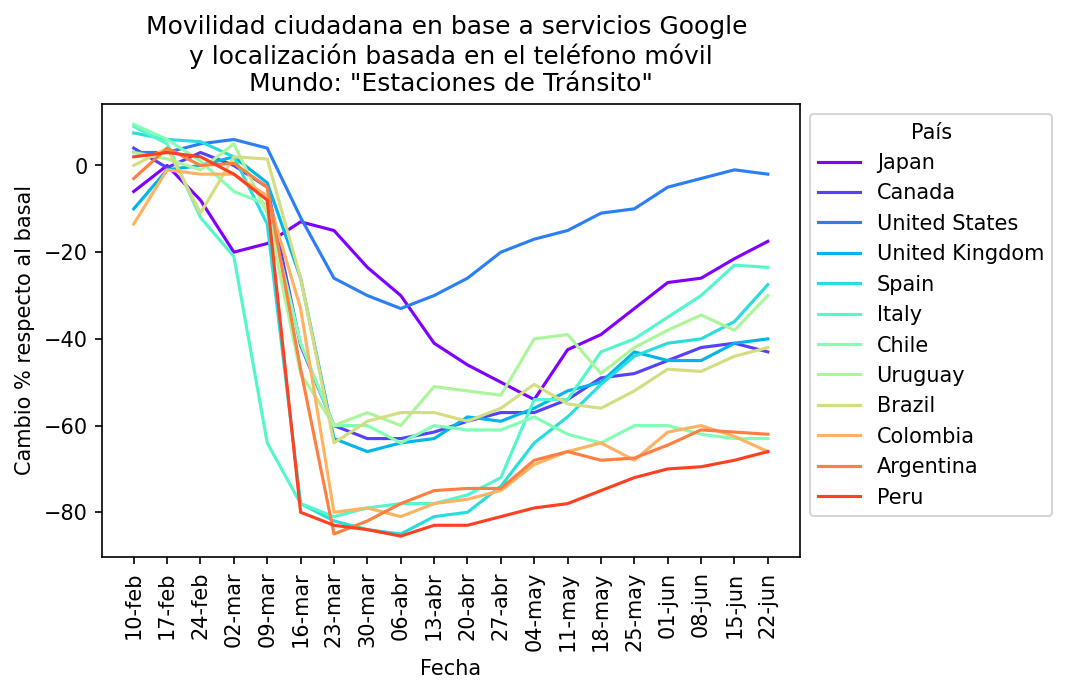
\includegraphics{./figtab/mundo_media.png} %%%%% grafo leído acá!!!
	\end{adjustbox}
	\caption{Movilidad ciudadana en la pandemia del Coronavirus19. Se presenta el indicador de movilidad basado en la cantidad visitas y duración de estas a varios tipos de localizaciones de algunos países de interés. Se muestra el cambio porcentual respecto a un basal y la mediana de la semana en el que se calcula el indicador. }
	\label{fig:movilidad mundial}
\end{figure}


\begin{table}[H]
	\begin{adjustbox}{width=1\textwidth}
		\input{./figtab/Movilidad_mundo_media.tab}   %%%%% tabla leída acá!!!
	\end{adjustbox}
	\caption{Movilidad ciudadana en la pandemia del Coronavirus19. Se presenta el indicador de movilidad basado en la cantidad visitas y duración de estas a varios tipos de localizaciones de algunos países de interés. Se muestra el cambio porcentual respecto a un basal y la mediana de la semana en el que se calcula el indicador. }
\label{tab:movilidad mundial}
\end{table}


%%%%% VARIANZA!!!
Cada país tuvo un comportamiento interno diferente, probablemente determinado por la fecha en que aparece el primer caso en el país o las medidas contra la pandemia de cada gobierno. Se presenta la desviación estandard de cada país a lo largo del tiempo, una medida de dispersión de las medidas de movilidad de cada país según cada semana en la figura \ref{fig:movilidad mundial_DS} y el gráfico \ref{tab:movilidad mundial_DS}.

\begin{figure}[H]
	\centering
	\begin{adjustbox}{width=0.8\textwidth}
		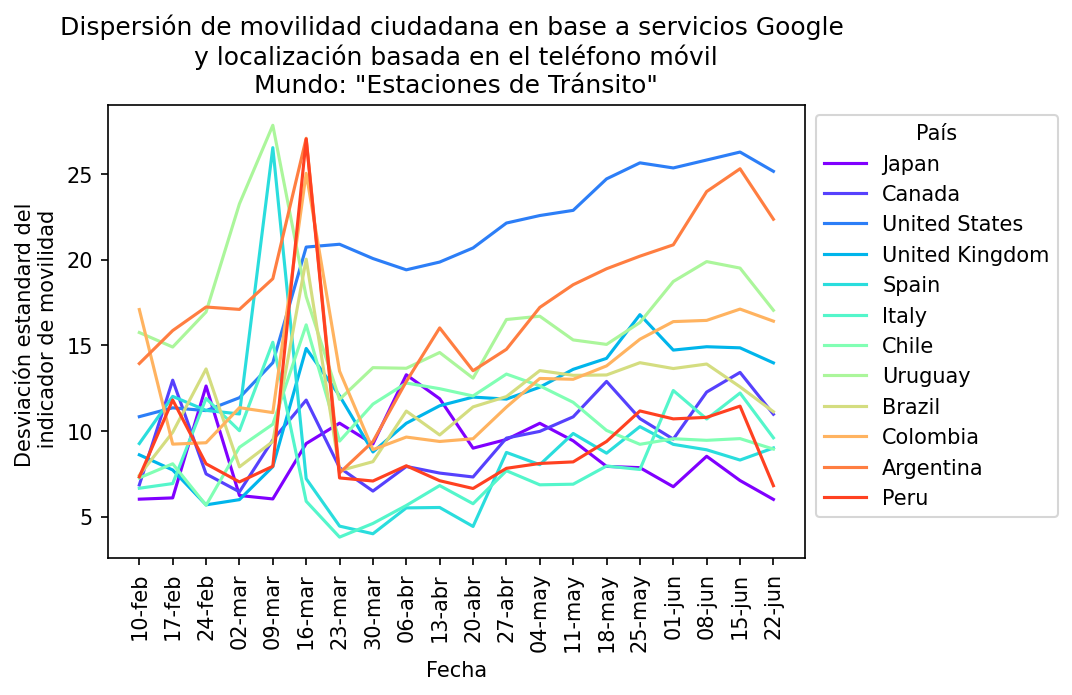
\includegraphics{./figtab/mundo_DS.png} %%%%% grafo leído acá!!!
	\end{adjustbox}
	\caption{Dispersión de la movilidad ciudadana en la pandemia del Coronavirus19. Se presenta la desviación estandard del indicador de movilidad basado en la cantidad visitas y duración de estas a varios tipos de localizaciones de algunos países de interés. Se muestra la desviación estandard de la movilidad ciudadana a lo largo del tiempo. }
	\label{fig:movilidad mundial_DS}
\end{figure}


\begin{table}[H]
	\begin{adjustbox}{width=1\textwidth}
		\input{./figtab/Movilidad_mundo_DS.tab}   %%%%% tabla leída acá!!!
	\end{adjustbox}
	\caption{Dispersión de la movilidad ciudadana en la pandemia del Coronavirus19. Se presenta el indicador de movilidad basado en la cantidad visitas y duración de estas a varios tipos de localizaciones de algunos países de interés. Se muestra la desviación estandard de la movilidad ciudadana a lo largo del tiempo.}
	\label{tab:movilidad mundial_DS}
\end{table}

\subsection{Visión local: Chile}

A continuación se presenta el análisis de los valores de movilidad ciudadana para Chile; la media semanal a lo largo del tiempo (figura \ref{fig:movilidad chile} y tabla \ref{tab:movilidad chile}) y la dispersión como desviación estandard de cada semana (figura \ref{fig:movilidad chile_DS} y tabla \ref{tab:movilidad chile_DS}) .


\begin{figure}[H]
	\centering
	\begin{adjustbox}{width=0.8\textwidth}
		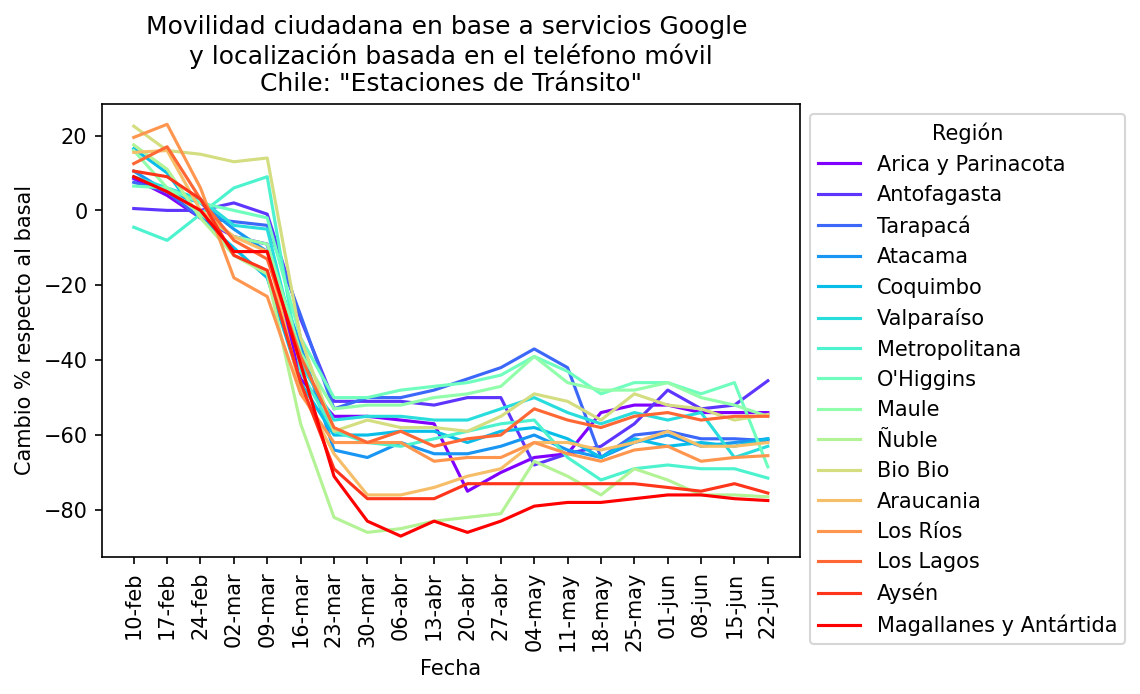
\includegraphics{./figtab/chile_media.png} %%%%% grafo leído acá!!!
	\end{adjustbox}
	\caption{Movilidad ciudadana en la pandemia del Coronavirus19. Se presenta el indicador de movilidad basado en la cantidad visitas y duración de estas a varios tipos de localizaciones de Chile. Se muestra el cambio porcentual respecto a un basal y la mediana de la semana en el que se calcula el indicador. }
	\label{fig:movilidad chile}
\end{figure}


\begin{table}[H]
	\begin{adjustbox}{width=1\textwidth}
		\input{./figtab/Movilidad_chile_media.tab}   %%%%% tabla leída acá!!!
	\end{adjustbox}
	\caption{Movilidad ciudadana en la pandemia del Coronavirus19. Se presenta el indicador de movilidad basado en la cantidad visitas y duración de estas a varios tipos de localizaciones de Chile. Se muestra el cambio porcentual respecto a un basal y la mediana de la semana en el que se calcula el indicador. }
	\label{tab:movilidad chile}
\end{table}


%%%%% VARIANZA!!!

\begin{figure}[H]
	\centering
	\begin{adjustbox}{width=0.8\textwidth}
		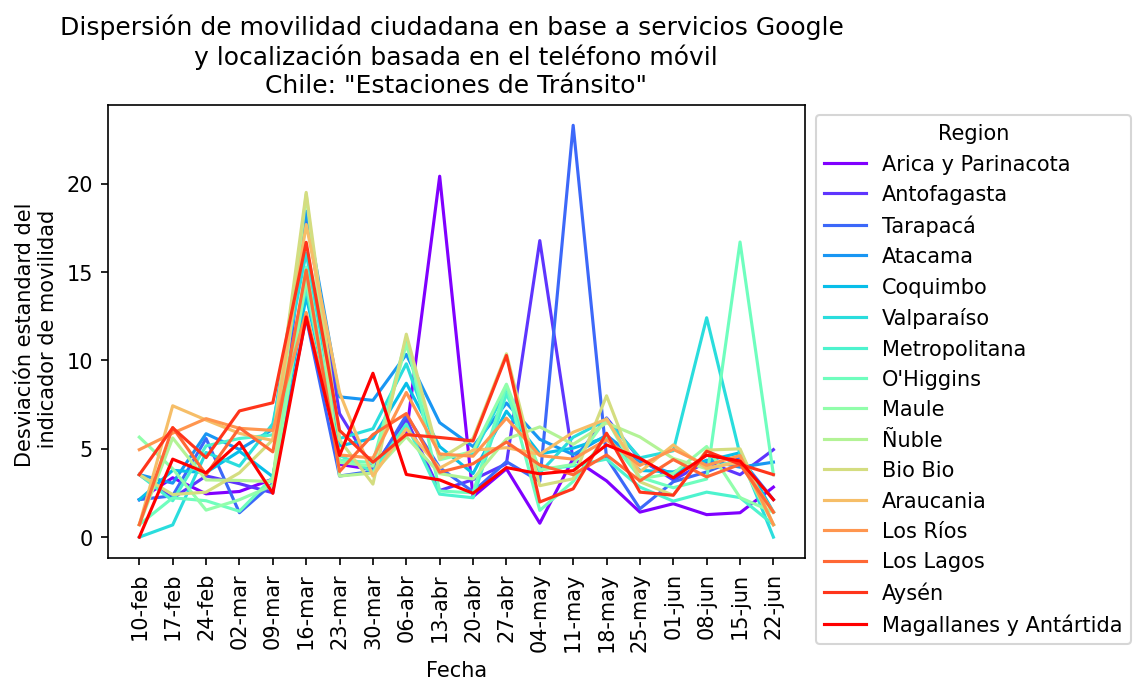
\includegraphics{./figtab/chile_DS.png} %%%%% grafo leído acá!!!
	\end{adjustbox}
	\caption{Movilidad ciudadana en la pandemia del Coronavirus19. Se presenta la desviación estandard del indicador de movilidad basado en la cantidad visitas y duración de estas a varios tipos de localizaciones de Chile. Se muestra la desviación estandard del cambio porcentual respecto a un basal y la mediana de la semana en el que se calcula el indicador. }
	\label{fig:movilidad chile_DS}
\end{figure}


\begin{table}[H]
	\begin{adjustbox}{width=1\textwidth}
		\input{./figtab/Movilidad_chile_DS.tab}   %%%%% tabla leída acá!!!
	\end{adjustbox}
	\caption{Movilidad ciudadana en la pandemia del Coronavirus19. Se presenta la desviación estandard del indicador de movilidad basado en la cantidad visitas y duración de estas a varios tipos de localizaciones de Chile. Se muestra la desviación estandard del cambio porcentual respecto a un basal y la mediana de la semana en el que se calcula el indicador. }
	\label{tab:movilidad chile_DS}
\end{table}



%%%%
%%%%  Las regiones
%%%%

\input{./textos/texto_region1.reg}

\input{./textos/texto_region2.reg}

\input{./textos/texto_region3.reg}

\input{./textos/texto_region4.reg}

\input{./textos/texto_region5.reg}

\input{./textos/texto_region6.reg}

\input{./textos/texto_region7.reg}

\input{./textos/texto_region8.reg}

\input{./textos/texto_region9.reg}

\input{./textos/texto_region10.reg}

\input{./textos/texto_region11.reg}

\input{./textos/texto_region12.reg}

\input{./textos/texto_region13.reg}

\input{./textos/texto_region14.reg}

\input{./textos/texto_region15.reg}

\input{./textos/texto_region16.reg}



\newpage
\bibliographystyle{vancouver}
\bibliography{bibliografia,Coronavirus_historia}



\end{document}